\documentclass{article}
\usepackage{kotex, verbatim}
\usepackage{amssymb,graphicx,verbatim,boxedminipage, subfigure,indentfirst}
\usepackage[left=2cm,right=2cm,top=2.54cm,bottom=2cm,a4paper]{geometry}
\usepackage[doublespacing]{setspace}

\title{프로그래밍 언어 hw3}
\author{B711016 김길호}
\date{\today}
\begin{document}
\maketitle
\newpage

\section{yacc란?}
    yacc란 내부에서 yylex(yyparse)함수를 호출하여 lex에서 인식한 토큰들을 넘겨받아 해당 토큰들의 관계를 분석한 후 구문 분석을 하는 구문 분석기입니다. 
    yacc를 사용하기위해서는 lex에서 토큰을 인식할 수 있어야하므로 어떤 토큰을 넘겨줄지에 대한 코드가 작성되어야 하고, lex에서 리턴하는 토큰 아이디들을
    이해하기 위해 lex의 결과 헤더파일을 include해야합니다. 또한 lex와 yacc가 통신하기 위해 yylval이라는 default값이 int인 미리 정의된 전역변수가 사용됩니다.
    yacc의 구조는 lex의 구조와 마찬가지로 크게 세 가지가 존재하며 두 개의 \%\%로 구분되어집니다. 
    \subsection{정의절}
        정의절은 \%\{과 \%\}으로 구분된 리터럴 블록과 (규칙절에서 사용할)변수 선언등을 담습니다. 리터럴 블록 내부에서는 
        c코드로 정의문과 같은 내용을 담을 수 있고, 변수 선언을 할 수 있습니다. 끝은 \%\%로 구분되고, 이는 lex파일에서의 정의절
        정의와 같습니다. 다만 토큰에 관계되는 데이터 타입을 등록하고 사용 할 수 있도록 \%union을 사용할 수 있고, \%token에 그 데이터 타입을 
        지정할 수 있습니다. 또한 토큰 아이디들은 yylex() 함수에서 리턴 값으로 사용 될 수도 있습니다.
    \subsection{규칙절}
        인식한 토큰들의 규칙 집합을 정의하는 부분입니다. 규칙은 (rule) : (symbole list) (action code); 꼴의 형태이며 c코드로 작성된 action을 실행한다는 면에선
        lex와 같은 구조로 보일 수 있으나 특정 토큰들이 이루는 symbole list가 모였을 때만 action code가 실행된다는 점, symbole list가 rule로 reduce되는
        점에서 lex와 다릅니다. 
        끝은 \%\%로 구분됩니다.
    \subsection{사용자 서브루틴절}
        yylex(yyparse)함수와 정의절에서 정의한 변수를 출력하는 등의 사용자가 원하는 C 루틴으로 구성되는 부분입니다. 이 또한 lex와 동일합니다.\\

\section{코드 분석 및 설명}
    설명은 카운팅 하는 부분에 대해 각각 섹션을 나눈 후, 각 섹션에 해당되는 내용을 카운트하기위해 어떤 token들이 어떤 rule들을 거쳐 reduce되어갔는지,
    필요한 경우 ansi문법 중 어느 부분을 고쳤는지, 카운트하기위해 어떤 변수들을 사용하였는지를 서술하고 설명을 위해 간단히 그린 파스트리 사진으로 
    파싱되는 과정을 보이겠습니다.
    코드는 token들이 reduce되는 과정을 모두 담기엔 너무 양이 방대하기에 핵심이 되는 부분만 기술하겠습니다.
        \subsection{Function}
        함수의 경우 선언, 정의, 사용하는 부분으로 크게 세 가지로 나눠서 생각할 수 있지만, 문제에서 함수의 정의가 항상 존재한다고 하였기에
        함수를 카운트 하는 곳은 정의,사용하는 부분과 예외적으로 포인터 함수를 정의하는 부분입니다. 
        먼저 아래 두 코드에서 함수가 정의, 사용되는 부분을 설명하고 포인터 함수 카운트하는 방법을 설명하겠습니다.\\
        \subsubsection{Normal func}
\begin{verbatim}
external_declaration    :   function_definition {kind = 0;ary[0]++;} // 일반적인 함수 (정의) 카운트 
postfix_expression      :   postfix_expression '(' ')' {ary[0]++;} // f()와 같은 argument가 없는 함수 (사용) 카운트
                        |   postfix_expression '(' argument_expression_list ')' {ary[0]++;} // f(a,b)와 같은 argument가 있는 함수 (사용) 카운트
\end{verbatim}

        \subsubsection{Pointer func}
            포인터 함수의 경우 아래와 같이 파스트리가 생성되었고, 두 가지 관찰을 통해 카운트 할 수 있었습니다.\\
            1. 먼저 괄호로 둘러쌓인 ptr, idenfier가 declarator로 reduce되므로 ptr가 나온다면 ptrfunc변수를 사용해 체크해줍니다. \\
            2. ( declarator ) 가 d.d로 reduce될 때 ptrfunc가 chk되어있다면 포인터 함수 이므로 이 때 카운트해주고 ptrfunc를 다시 초기화합니다.\\
        \begin{figure}[h]
            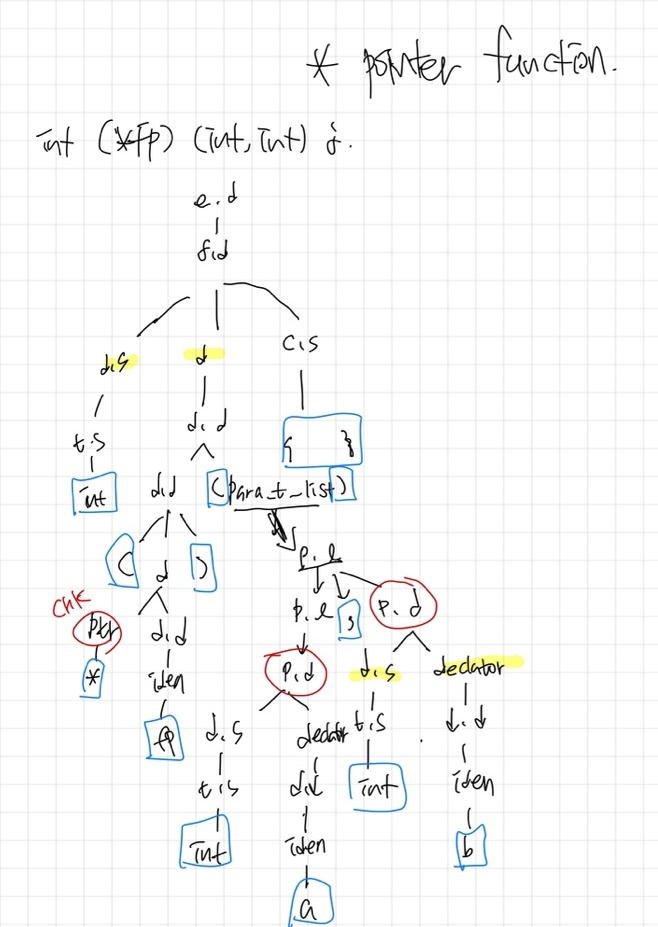
\includegraphics[width = 0.3\textwidth]{ptrfun.jpg}
        \end{figure}
\newpage
\begin{verbatim}
declarator        : pointer direct_declarator{
                    ptrfunc = 1; 
                    ary[4]++;} 
direct_declarator : '(' declarator ')' {if (ptrfunc) ary[0]++, ptrfunc=0;}
\end{verbatim}     

        \subsection{Operator}
            연산자의 경우 lex에서 해당하는 토큰의 이름을 넘겨주었기에 PTR\_OP, INC\_OP, $".", "->"$ 등과 같이 해당하는 부분들을 찾아 각각 카운트해줬습니다. 
            이 부분은 단순 나열된 문장들을 찾은 것이기에 이곳엔 작성하지않을 것이고, 마지막 전체코드를 통해 확인할 수 있습니다.
            다만 대입연산자의 경우 assignment\_expression으로 reduce되는 경우 밖에 없었기에 assignment\_operator을 각각 카운트 하지않고 reduce될 때 한번 카운트 해줬습니다.
\begin{verbatim}
assignment_expression   | unary_expression assignment_operator assignment_expression {ary[1]++;}
\end{verbatim}   

        \subsection{Int, Char}
            int와 char의 경우 자료형만 다르고 카운트 해야하는 부분은 같기에 묶어서 서술하겠습니다. 두 자료형 모두 선언된 자료형을 갖는 변수(매개변수, 구조체 내 변수) 개수를 카운트하는것이었기에
            우선 int, char토큰을 받을 때마다 그 종류를 저장할 변수(kind)를 이용하여 관리할 수 있었습니다. 이 문제도 간단히 파스트리를 그려 어디서 카운트해야했는지 생각해봤습니다.\\\\
            1. 파라미터의 매개변수에선 (자료형, 변수)가 토큰으로 인식된 declaration\_specifiers declarator이 parameter\_declaration으로 reduce될 때, declaration\_specifiers에서 저장해놓은 
            kind의 값에 따라 -1이면 int를 1이면 char, 나머지는 0으로 인식할 수 있었고 결과적으로 kind의 값이 -1, 1일 때만 카운트한 뒤, kind를 0으로 초기화해주었습니다.\\\\
            2. 파라미터에서가 아닌 변수 선언에 대해서는 단일 변수선언과 ,로 나열된 변수 선언으로 두 가지 상황이 존재했는데 파스트리에서 보면 전자의 경우 init\_declarator에서 init\_declarator\_list으로
            reduce, 후자의 경우 init\_declarator\_list ',' init\_declarator에서 init\_declarator\_list으로 reduce될 때 kind의 값을 체크한 후 카운트해주면 됐습니다. 이 때 2번에서는 kind를 즉각 초기화
            해줬지만 선언문에서 ,로 나열되는 경우 선언문의 자료형이 한 개이기떄문에 kind를 바로 초기화하지않고 declaration\_specifiers init\_declarator\_list이 declaration으로 reduce될 때 0으로 초기화해주었습니다.\\\\
            3. struct 구조체에 선언된 변수의 경우 (자료형, 변수)가 각각 specifier\_qualifier\_list struct\_declarator\_list으로 인식되었고, 2에서 변수 선언한 방식과 동일한 방식으로 변수가 선언되었는데
            ,로 나열된 변수는 struct\_declarator\_list ',' struct\_declarator 이 struct\_declarator\_list으로 reduce, 단일 변수 선언의 경우 struct\_declarator이 struct\_declarator\_list으로 reduce될 때 
            kind의 값을 확인하고 카운트해주면 됐습니다.\\
            \newpage
        \begin{figure}[h]
            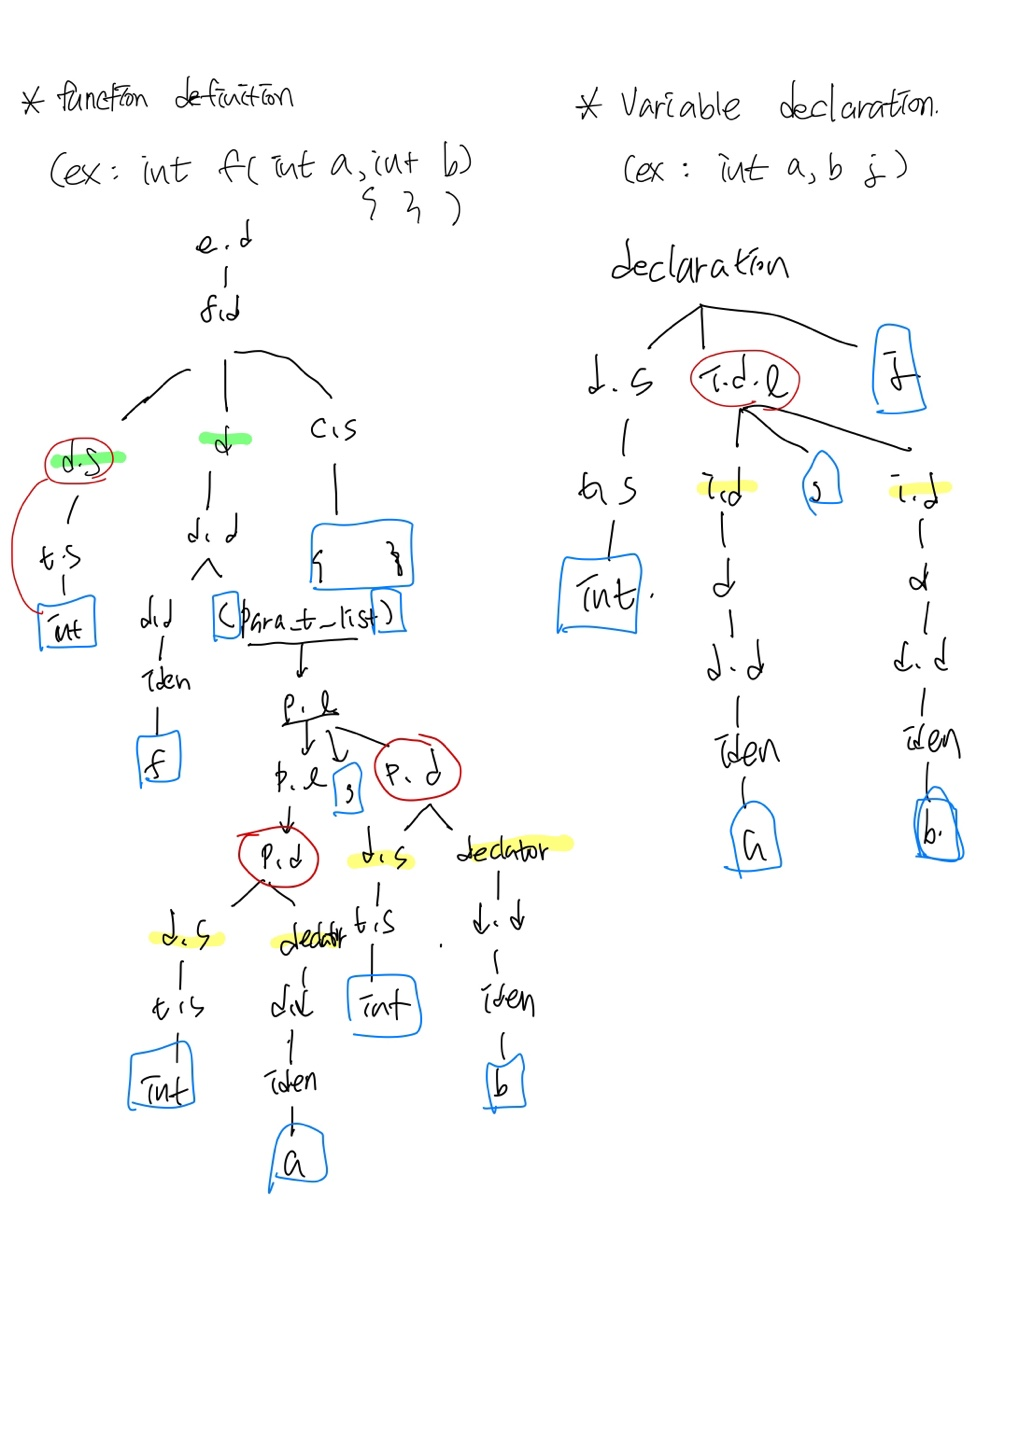
\includegraphics[width = 0.3\textwidth]{func_vari_def.jpg}
        \end{figure}
        
\begin{verbatim}
init_declarator_list    :   init_declarator {
                                if (kind == -1) {ary[2]++;} 
                                else if (kind == 1) {ary[3]++;}
                            }
	                        |   init_declarator_list ',' init_declarator {
		                                if (kind == -1) {ary[2]++;} 
		                                else if (kind == 1) {ary[3]++;}
	                            }
type_specifier      : VOID {kind = 0;}
	                    | CHAR {kind = 1;}
	                    | SHORT {kind = 0;}
	                    | INT {kind = -1;}
	                    | LONG {kind = 0;}
	                    | FLOAT {kind = 0;}
	                    | DOUBLE {kind = 0;}
	                    | SIGNED {kind = 0;}
	                    | UNSIGNED {kind = 0;}
	                    | struct_or_union_specifier {kind = 0;}
	                    | enum_specifier {kind = 0;}
	                    | TYPE_NAME {kind = 0;}
struct_declarator_list  : struct_declarator {
		                        if (kind == -1) {ary[2]++;} 
		                        else if (kind == 1) {ary[3]++;}
	                    }
	                    | struct_declarator_list ',' struct_declarator {
		                        if (kind == -1) {ary[2]++;} 
		                        else if (kind == 1) {ary[3]++;}
	                    }
parameter_declaration   : declaration_specifiers declarator {
		                        if (kind == -1) {ary[2]++; } 
		                        else if (kind == 1) {ary[3]++; }
		                        kind = 0; 
	                    }
	                    | declaration_specifiers abstract_declarator {kind = 0;}
	                    | declaration_specifiers {kind = 0;}
	;
\end{verbatim}
\newpage
    \subsection{Pointer}
        Pointer의 경우 '*'으로 받은 토큰이 pointer로 reduce되고, pointer에서 reduce된 선언 문은 한 줄 밖에 없었기에 pointer direct\_declarator에서 declarator으로 
        reduce될 때 이를 카운트했습니다. (pointer에서 카운트하지않은 이유는 더블 포인터같은 여러개의 포인터가 있는 경우 중복되어 카운트되기 때문입니다.)
\begin{verbatim}
declarator        : pointer direct_declarator{ ptrfunc = 1; ary[4]++;} 
\end{verbatim}
    \subsection{Array}
        Array의 경우 선언된 배열의 개수를 세야하는 것이므로 declarator부근에서 [, ]가 파싱되는 부분을 찾아 카운트하려했습니다. 하지만 이와 같이 카운트하면 다차원 배열
        에서 카운트가 누적되기때문에 direct\_declarator '[' constant\_expression ']'에서 direct\_declarator으로 reduce될 때와 direct\_declarator '[' ']'에서 direct\_declarator으로 reduce될 때
        배열 선언이 일어났다는 걸 표시할 변수 many\_dim을 사용해 체크한 후, direct\_declarator에서 declarator으로 reduce되기 전 many\_dim이 체크되어있으면 카운트해주고 many\_dim을 초기화해주었습니다.\\
        \begin{figure}[h]
            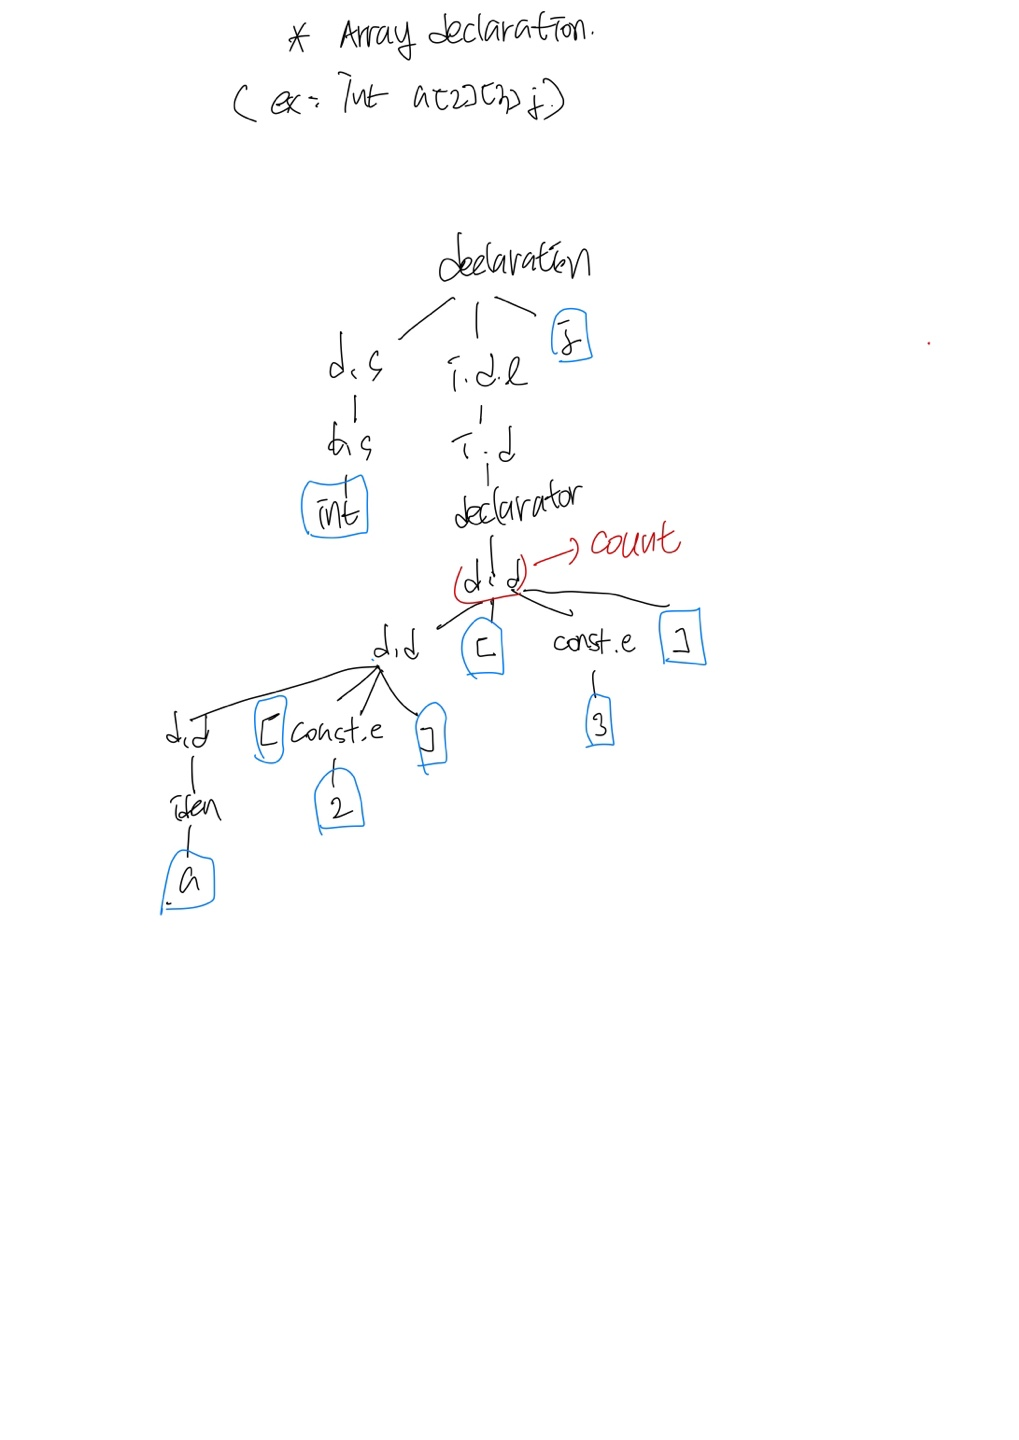
\includegraphics[width = 0.3\textwidth]{ary.jpg}
        \end{figure}
\begin{verbatim}
declarator          |   direct_declarator {if(many_dim) ary[5]++; many_dim = 0;}
direct_declarator   |   direct_declarator '[' constant_expression ']' { many_dim = 1;}  
	                    |   direct_declarator '[' ']' { many_dim = 1;} 
\end{verbatim}
    \subsection{Selection}
        ansi문법을 그대로 가져와서 썼을 때, if else 구문과 if 구문의 conflict충돌이 일어났는데 이는 if 토큰을 인식했을 때 일어나는 모호성때문에 발생한 문제였습니다.
        이와 관련해서 아래와 같은 우선순위를 지정해줘서 if else의 우선순위를 더 높게 인식하도록 설정하였습니다.\begin{verbatim}%nonassoc LOWER_THEN_ELSE , %nonassoc ELSE \end{verbatim} \\
        이에 카운트를 할 때는 문제에서 if문만 주어진다고 가정하였기에 if, switch 구문을 만났을 때 이를 체크할 findslc변수를 사용하였고, 각 구문이 selection\_statement로 reduce
        , selection\_statement에서 statement로 reduce 될 때 findslc변수의 체크 여부에 따라 카운트한 후 findslc변수를 초기화해줬습니다.
\begin{verbatim}
statement           |   selection_statement {if(findslc) ary[6]++; findslc=0;}
selection_statement :   IF '(' expression ')' statement %prec LOWER_THEN_ELSE 	{findslc = 1;}
            	        |   SWITCH '(' expression ')'   statement {findslc = 1;}
\end{verbatim}
    \subsection{Iteration}
        반복문은 iteration\_statement으로 reduce되는 부분을 찾아 각각 카운트해줬습니다. 이때 ansi문법을 그대로 가져다쓸경우 for문안에 변수선언이 불가능하였기에 이를 처리할 수 있도록
        iteraton\_statement로 reduce되는 부분쪽에 아래 두 구문을 추가하여 해결하였습니다.
        \begin{verbatim} FOR '(' declaration expression_statement ')' statement, FOR '(' declaration expression_statement expression ')' statement \end{verbatim}
\begin{verbatim}
iteration_statement
	: WHILE '(' expression ')' statement		{ ary[7]++;}
	| DO statement WHILE '(' expression ')' ';' { ary[7]++;}
	| FOR '(' expression_statement expression_statement ')' statement { ary[7]++;}
	| FOR '(' expression_statement expression_statement expression ')' statement { ary[7]++;} 
	| FOR '(' declaration expression_statement ')' statement { ary[7]++;}
	| FOR '(' declaration expression_statement expression ')' statement { ary[7]++;} 

\end{verbatim}
    \subsection{Return}
        리턴문의 경우 "return" 토큰으로 넘겨받았을 때, 일반적으로 두 가지 경우를 생각할 수 있습니다. 첫번째는 return ; 과 같이 반환 타입이 없는 경우이고, 두 번째는 return ();과 같이 ()안에 expression(수식이나 값 또는 변수)으로 reduce된 토큰과 함께 존재할 수 있습니다.
        따라서 위의 두 가지 경우에 해당되는 경우만 카운트했습니다. (printf("return;")의 경우 "return;..." 가 따옴표로 둘러싸인 string\_literal로 reduce되고 결국 postfix\_expression으로 reduce되기에 카운팅되지않습니다.)
\begin{verbatim}
jump_statement
	| RETURN ';' {ary[8]++;} 
	| RETURN expression ';' {ary[8]++;} 
\end{verbatim}
\newpage
    \subsection{변수 선언 위치 자유}
        변수 선언 위치는 받은 ansi문법부분에서 compound\_statement와 declaration\_list 관련해서 생기는 문제였습니다. 최신 ansi문법을 참고하여 declaration\_list심볼을 뒤로 배치해주었고, compound\_statement도 약간 고쳐서 해결할 수 있었습니다.\\
\begin{verbatim}
compound_statement
	: '{' '}'
	| '{'  block_item_list '}'
	;

block_item_list
	: block_item
	| block_item_list block_item
	;

block_item
	: declaration
	| statement
	;
declaration_list
	: declaration
	| declaration_list declaration
	;
\end{verbatim}
    \subsection{서술하지않은 부분}
        1. define, include와 같은 전처리문은 이 전 lex과제에서 사용했던 코드를 재사용했습니다.
        이는 lex에서 아래와 같이 코드를 작성하였는데 헤더 include하는 부분은 yacc에서 카운팅할 때 아무 의미가 없으므로 해당 구문을 전부 무시하게하였고,
        define하는 부분은 어떤 문자를 상수로 define한다해도 어차피 yacc에서 문자를 처리하는 부분에서 일어날 수 있는 모든 상황에 idenfier로 존재할 수 있기에
        define구문도 무시하게 처리하였습니다. 
        \begin{verbatim}"#include".*\n	{;}, "#define".*\n	{;}\end{verbatim} 
        \newpage
        2. 주석문도 마찬가지로 lex과제에서 사용했던 코드를 재사용했습니다. 
        이는 단일 주석과 여러 줄의 주석을 처리할 때 단일 주석은 그냥 무시하게하였고, 여러 줄의 주석을 처리할 때는 여는 주석을 만났을 때 
        지정해둔 곳(COMMENT)으로 분기하며 닫는 괄호를 만날 때까지 있는 모든 문자를 무시합니다. 결과적으로 닫는 괄호가 나온다면 다시 처음으로 돌아가도록하여 두 주석 모두 깔끔하게 처리할 수 있습니다.   
        \begin{verbatim}
        %x COMMENT
        %%
        "/*"	{BEGIN(COMMENT);} 
        "//".*	{;} 
        
        <COMMENT>.|\n	;
        <COMMENT>"*/"	{BEGIN(INITIAL);}
        \end{verbatim}

\section{Yacc Code}
\begin{verbatim}
%{
#include <stdio.h>
#include <string.h>

int ary[9] = {0,0,0,0,0,0,0,0,0};

int kind = 0; // -1 : int , 0 : other, 1 : char
int many_dim = 0;
int ptrfunc = 0;
int findslc = 0;

%}

%token IDENTIFIER CONSTANT STRING_LITERAL SIZEOF
%token PTR_OP INC_OP DEC_OP LEFT_OP RIGHT_OP LE_OP GE_OP EQ_OP NE_OP
%token AND_OP OR_OP MUL_ASSIGN DIV_ASSIGN MOD_ASSIGN ADD_ASSIGN
%token SUB_ASSIGN LEFT_ASSIGN RIGHT_ASSIGN AND_ASSIGN
%token XOR_ASSIGN OR_ASSIGN TYPE_NAME

%token TYPEDEF EXTERN STATIC AUTO REGISTER
%token CHAR SHORT INT LONG SIGNED UNSIGNED FLOAT DOUBLE CONST VOLATILE VOID
%token STRUCT UNION ENUM ELLIPSIS

%token CASE DEFAULT IF ELSE SWITCH WHILE DO FOR GOTO CONTINUE BREAK RETURN
%nonassoc LOWER_THEN_ELSE
%nonassoc ELSE
%start translation_unit
%%

primary_expression
	: IDENTIFIER 
	| CONSTANT 
	| STRING_LITERAL 
	| '(' expression ')' 
	;

postfix_expression
	: primary_expression 
	| postfix_expression '[' expression ']' 
	| postfix_expression '(' ')' {ary[0]++;}
	| postfix_expression '(' argument_expression_list ')' {ary[0]++;}
	| postfix_expression '.' IDENTIFIER {ary[1]++;} 
	| postfix_expression PTR_OP IDENTIFIER {ary[1]++;} 
	| postfix_expression INC_OP {ary[1]++;}
	| postfix_expression DEC_OP {ary[1]++;}
	;

argument_expression_list
	: assignment_expression
	| argument_expression_list ',' assignment_expression
	;

unary_expression
	: postfix_expression 
	| INC_OP unary_expression {ary[1]++;}
	| DEC_OP unary_expression {ary[1]++;}
	| unary_operator cast_expression   
	| SIZEOF unary_expression  
	| SIZEOF '(' type_name ')'
	;

unary_operator
	: '&'
	| '*'
	| '+'
	| '-'
	| '~'
	| '!'
	;

cast_expression
	: unary_expression 
	| '(' type_name ')' cast_expression {ary[1]++;}
	;

multiplicative_expression
	: cast_expression 
	| multiplicative_expression '*' cast_expression {ary[1]++;}	
	| multiplicative_expression '/' cast_expression {ary[1]++;}	
	| multiplicative_expression '%' cast_expression {ary[1]++;}	
	;

additive_expression
	: multiplicative_expression
	| additive_expression '+' multiplicative_expression {ary[1]++;}	
	| additive_expression '-' multiplicative_expression {ary[1]++;}	
	;

shift_expression
	: additive_expression
	| shift_expression LEFT_OP additive_expression	{ ary[1]++;}	
	| shift_expression RIGHT_OP additive_expression	{ ary[1]++;}	
	;

relational_expression
	: shift_expression
	| relational_expression '<' shift_expression {ary[1]++;}	
	| relational_expression '>' shift_expression {ary[1]++;}	
	| relational_expression LE_OP shift_expression { ary[1]++;}	
	| relational_expression GE_OP shift_expression { ary[1]++;}	
	;

equality_expression
	: relational_expression
	| equality_expression EQ_OP relational_expression { ary[1]++;}	
	| equality_expression NE_OP relational_expression { ary[1]++;}	
	;

and_expression
	: equality_expression
	| and_expression '&' equality_expression {ary[1]++;}	
	;

exclusive_or_expression
	: and_expression
	| exclusive_or_expression '^' and_expression {ary[1]++;}	
	;

inclusive_or_expression
	: exclusive_or_expression
	| inclusive_or_expression '|' exclusive_or_expression {ary[1]++;}	
	;

logical_and_expression
	: inclusive_or_expression
	| logical_and_expression AND_OP inclusive_or_expression {ary[1]++;}	
	;

logical_or_expression
	: logical_and_expression
	| logical_or_expression OR_OP logical_and_expression {ary[1]++;}	
	;

conditional_expression
	: logical_or_expression
	| logical_or_expression '?' expression ':' conditional_expression
	;

assignment_expression
	: conditional_expression 
	| unary_expression assignment_operator assignment_expression {ary[1]++;}
	;

assignment_operator
	: '=' 
	| MUL_ASSIGN
	| DIV_ASSIGN
	| MOD_ASSIGN
	| ADD_ASSIGN
	| SUB_ASSIGN
	| LEFT_ASSIGN
	| RIGHT_ASSIGN
	| AND_ASSIGN
	| XOR_ASSIGN
	| OR_ASSIGN
	;

expression
	: assignment_expression
	| expression ',' assignment_expression
	;

constant_expression
	: conditional_expression 
	;

declaration
	: declaration_specifiers ';' {kind = 0;}
	| declaration_specifiers init_declarator_list ';' {kind = 0;}
	;

declaration_specifiers
	: storage_class_specifier declaration_specifiers 
	| storage_class_specifier 
	| type_specifier declaration_specifiers 
	| type_specifier 
	| type_qualifier declaration_specifiers
	| type_qualifier 
	;

init_declarator_list
	: init_declarator {
		if (kind == -1) {ary[2]++;} 
		else if (kind == 1) {ary[3]++;}
	}
	| init_declarator_list ',' init_declarator {
		if (kind == -1) {ary[2]++;} 
		else if (kind == 1) {ary[3]++;}
	}
	;

init_declarator
	: declarator 
	| declarator '=' initializer {ary[1]++;}
	;

storage_class_specifier
	: TYPEDEF {kind = 0;}
	| EXTERN {kind = 0;}
	| STATIC {kind = 0;}
	| AUTO {kind = 0;}
	| REGISTER {kind = 0;}
	;

type_specifier
	: VOID {kind = 0;}
	| CHAR {kind = 1;}
	| SHORT {kind = 0;}
	| INT {kind = -1;}
	| LONG {kind = 0;}
	| FLOAT {kind = 0;}
	| DOUBLE {kind = 0;}
	| SIGNED {kind = 0;}
	| UNSIGNED {kind = 0;}
	| struct_or_union_specifier {kind = 0;}
	| enum_specifier {kind = 0;}
	| TYPE_NAME {kind = 0;}
	;

struct_or_union_specifier
	: struct_or_union '{' struct_declaration_list '}' 
	| struct_or_union IDENTIFIER '{' struct_declaration_list '}' 
	| struct_or_union IDENTIFIER 
	;

struct_or_union
	: STRUCT 
	| UNION 
	;

struct_declaration_list
	: struct_declaration 
	| struct_declaration_list struct_declaration 
	;

struct_declaration
	: specifier_qualifier_list struct_declarator_list ';' {kind = 0;}
	;

specifier_qualifier_list
	: type_specifier specifier_qualifier_list 
	| type_specifier 
	| type_qualifier specifier_qualifier_list 
	| type_qualifier 
	;

struct_declarator_list
	: struct_declarator {
		if (kind == -1) {ary[2]++;} 
		else if (kind == 1) {ary[3]++;}
	}
	| struct_declarator_list ',' struct_declarator {
		if (kind == -1) {ary[2]++;} 
		else if (kind == 1) {ary[3]++;}
	}
	;

struct_declarator
	: declarator 
	| ':' constant_expression 
	| declarator ':' constant_expression 
	;

enum_specifier
	: ENUM '{' enumerator_list '}'
	| ENUM IDENTIFIER '{' enumerator_list '}'
	| ENUM IDENTIFIER
	;

enumerator_list
	: enumerator
	| enumerator_list ',' enumerator
	;

enumerator
	: IDENTIFIER
	| IDENTIFIER '=' constant_expression {ary[1]++;}	
	;

type_qualifier
	: CONST
	| VOLATILE
	;

declarator
	: pointer direct_declarator {
		ptrfunc = 1; 
		ary[4]++;
		} 
	| direct_declarator {
		if(many_dim) ary[5]++; 
		many_dim = 0;  
		}
	;

direct_declarator
	: IDENTIFIER 
	| '(' declarator ')' {if (ptrfunc) ary[0]++, ptrfunc=0; }
	| direct_declarator '[' constant_expression ']' { many_dim = 1; }  
	| direct_declarator '[' ']' { many_dim = 1; } 
	| direct_declarator '(' parameter_type_list ')' 
	| direct_declarator '(' identifier_list ')' 
	| direct_declarator '(' ')' 
	;

pointer
	: '*'
	| '*' type_qualifier_list
	| '*' pointer
	| '*' type_qualifier_list pointer
	;

type_qualifier_list
	: type_qualifier
	| type_qualifier_list type_qualifier
	;


parameter_type_list
	: parameter_list 
	| parameter_list ',' ELLIPSIS
	;

parameter_list
	: parameter_declaration 
	| parameter_list ',' parameter_declaration 
	;

parameter_declaration
	: declaration_specifiers declarator {
		if (kind == -1) {ary[2]++; } 
		else if (kind == 1) {ary[3]++; }
		kind = 0; 
	  }
	| declaration_specifiers abstract_declarator {kind = 0;}
	| declaration_specifiers {kind = 0;}
	;

identifier_list
	: IDENTIFIER 
	| identifier_list ',' IDENTIFIER 
	;

type_name
	: specifier_qualifier_list
	| specifier_qualifier_list abstract_declarator
	;

abstract_declarator
	: pointer
	| direct_abstract_declarator
	| pointer direct_abstract_declarator
	;

direct_abstract_declarator
	: '(' abstract_declarator ')'
	| '[' ']'
	| '[' constant_expression ']'
	| direct_abstract_declarator '[' ']'
	| direct_abstract_declarator '[' constant_expression ']'
	| '(' ')'
	| '(' parameter_type_list ')'
	| direct_abstract_declarator '(' ')'
	| direct_abstract_declarator '(' parameter_type_list ')'
	;

initializer
	: assignment_expression
	| '{' initializer_list '}'
	| '{' initializer_list ',' '}'
	;

initializer_list
	: initializer
	| initializer_list ',' initializer
	;

statement
	: labeled_statement
	| compound_statement
	| expression_statement
	| selection_statement {if(findslc) ary[6]++; findslc=0;}
	| iteration_statement
	| jump_statement 
	;

labeled_statement
	: IDENTIFIER ':' statement
	| CASE constant_expression ':' statement
	| DEFAULT ':' statement
	;

compound_statement
	: '{' '}'
	| '{'  block_item_list '}'
	;

block_item_list
	: block_item
	| block_item_list block_item
	;

block_item
	: declaration
	| statement
	;

expression_statement
	: ';'
	| expression ';'
	;

selection_statement
	: IF '(' expression ')' statement %prec LOWER_THEN_ELSE 	{findslc = 1;}
	| IF '(' expression ')' statement ELSE statement			
	| SWITCH '(' expression ')' statement 						{findslc = 1;}
	;

iteration_statement
	: WHILE '(' expression ')' statement		{ary[7]++;}
	| DO statement WHILE '(' expression ')' ';' {ary[7]++;}
	| FOR '(' expression_statement expression_statement ')' statement {ary[7]++;}
	| FOR '(' expression_statement expression_statement expression ')' statement {ary[7]++;} 
	| FOR '(' declaration expression_statement ')' statement {ary[7]++;}
	| FOR '(' declaration expression_statement expression ')' statement {ary[7]++;} 
	;

jump_statement
	: GOTO IDENTIFIER ';'
	| CONTINUE ';'
	| BREAK ';'
	| RETURN ';' {ary[8]++;} 
	| RETURN expression ';' {ary[8]++;} 
	;

translation_unit
	: external_declaration
	| translation_unit external_declaration
	;

external_declaration 
	: function_definition {kind = 0;ary[0]++; }
	| declaration {kind = 0;}		 
	;

function_definition
	: declaration_specifiers declarator declaration_list compound_statement {kind = 0;}
	| declaration_specifiers declarator compound_statement {kind = 0;}
	| declarator declaration_list compound_statement 
	| declarator compound_statement 
	;

declaration_list
	: declaration
	| declaration_list declaration
	;

%%

int main(void)
{
	yyparse();

	printf("function = %d\n", ary[0]);
	printf("operator = %d\n", ary[1]);
	printf("int = %d\n", ary[2]);
	printf("char = %d\n", ary[3]);
	printf("pointer = %d\n", ary[4]);
	printf("array = %d\n", ary[5]);
	printf("selection = %d\n", ary[6]);
	printf("loop = %d\n", ary[7]);
	printf("return = %d\n", ary[8]);
	return 0;
}

void yyerror(const char *str)
{
	fprintf(stderr, "error: %s\n", str);
}

\end{verbatim}
\end{document}